\documentclass[a4paper,12pt]{article}
\usepackage[utf8]{inputenc}
\usepackage[T1]{fontenc}
\usepackage[brazilian]{babel}
\usepackage{amsmath}
\usepackage{graphicx}
\usepackage{float}
\usepackage{booktabs}
\usepackage{listings}
\usepackage{xcolor}
\usepackage{geometry}
\geometry{margin=2.5cm}

\definecolor{codegreen}{rgb}{0,0.6,0}
\definecolor{codegray}{rgb}{0.5,0.5,0.5}
\definecolor{codepurple}{rgb}{0.58,0,0.82}
\definecolor{backcolour}{rgb}{0.95,0.95,0.92}

\lstset{
    backgroundcolor=\color{backcolour},   
    commentstyle=\color{codegreen},
    keywordstyle=\color{magenta},
    numberstyle=\tiny\color{codegray},
    stringstyle=\color{codepurple},
    basicstyle=\ttfamily\footnotesize,
    breakatwhitespace=false,         
    breaklines=true,                 
    captionpos=b,                    
    keepspaces=true,                 
    numbers=left,                    
    numbersep=5pt,                  
    showspaces=false,                
    showstringspaces=false,
    showtabs=false,                  
    tabsize=2,
    language=C,
    extendedchars=true,
    literate={á}{{\'a}}1 {à}{{\`a}}1 {ã}{{\~a}}1 {é}{{\'e}}1 {ê}{{\^e}}1 {í}{{\'i}}1 {ó}{{\'o}}1 {õ}{{\~o}}1 {ú}{{\'u}}1 {ç}{{\c{c}}}1 {Á}{{\'A}}1 {À}{{\`A}}1 {Ã}{{\~A}}1 {É}{{\'E}}1 {Ê}{{\^E}}1 {Í}{{\'I}}1 {Ó}{{\'O}}1 {Õ}{{\~O}}1 {Ú}{{\'U}}1 {Ç}{{\c{C}}}1
}

\title{Relatório Tarefa 3: Implementação, Análise de Convergência e Custo Computacional no Cálculo de Pi}
\author{Thiago Jordão}
\date{\today}

\begin{document}

\maketitle

\section{Introdução}

O objetivo desta experiência foi implementar e analisar algoritmos em linguagem C capazes de calcular aproximações da constante matemática $\pi$. O foco do estudo é avaliar o compromisso (\textit{trade-off}) entre o tempo de processamento, o número de iterações e a precisão do resultado final, comparando duas abordagens matemáticas distintas.

Foram implementadas duas soluções:

\begin{enumerate}
    \item \textbf{Série de Gregory-Leibniz:} Uma série infinita clássica e de implementação direta:
    \[\pi = 4 \sum_{n=0}^{\infty} \frac{(-1)^n}{2n+1}\]

    \item \textbf{Fórmula de Machin (1706):} Uma abordagem otimizada que utiliza a expansão da Série de Taylor para a função arco-tangente:
    \[\frac{\pi}{4} = 4 \arctan\left(\frac{1}{5}\right) - \arctan\left(\frac{1}{239}\right)\]
\end{enumerate}

\section{Metodologia}

Os programas foram desenvolvidos na linguagem C, aferindo o tempo de CPU por meio da biblioteca \texttt{<time.h>} (\texttt{clock\_t}) e calculando o erro absoluto com base na constante \texttt{M\_PI} da biblioteca \texttt{<math.h>}. Os códigos-fonte completos encontram-se na secção de Anexos no final deste documento.

Para a Série de Leibniz, os testes variaram de 10 a 1.000.000.000 de iterações. Para a Fórmula de Machin, dada a sua característica matemática, os testes exploraram um espetro menor, de 1 a 10.000.000 de iterações. Todos os cálculos utilizaram o tipo \texttt{double} para garantir dupla precisão em vírgula flutuante.

\section{Resultados e Análise Comparativa}

\begin{table}[H]
\centering
\caption{Convergência pela Série de Leibniz}
\begin{tabular}{@{}llll@{}}
\toprule
Iterações & Tempo (s) & Valor Estimado & Erro Absoluto \\ \midrule
10 & 0.000005 & 3.0418396189 & 0.0997530347 \\
100 & 0.000001 & 3.1315929036 & 0.0099997500 \\
10.000 & 0.000019 & 3.1414926536 & 0.0001000000 \\
1.000.000 & 0.001634 & 3.1415916536 & 0.0000010000 \\
100.000.000 & 0.188943 & 3.1415926436 & 0.0000000100 \\
1.000.000.000 & 1.845652 & 3.1415926526 & 0.0000000010 \\ \bottomrule
\end{tabular}
\end{table}

\begin{table}[H]
\centering
\caption{Convergência pela Fórmula de Machin}
\begin{tabular}{@{}llll@{}}
\toprule
Iterações & Tempo (s) & Valor Estimado & Erro Absoluto \\ \midrule
1 & 0.000002 & 3.1832635983 & 0.0416709447 \\
2 & 0.000001 & 3.1405970293 & 0.0009956243 \\
5 & 0.000001 & 3.1415926824 & 0.0000000288 \\
10 & 0.000001 & 3.1415926536 & 0.0000000000 \\
10.000.000 & 0.059722 & 3.1415926536 & 0.0000000000 \\ \bottomrule
\end{tabular}
\end{table}

\textbf{Análise do Custo vs. Precisão:}
Os dados empíricos demonstram claramente a diferença entre depender do poder de processamento bruto e utilizar a otimização matemática adequada:

\begin{itemize}
    \item \textbf{Comportamento Linear vs. Exponencial:} A série de Leibniz (Tabela 1) apresenta uma convergência extremamente lenta. Para reduzir o erro absoluto num fator de 10 (ganhar uma casa decimal de precisão), é estritamente necessário multiplicar o número de iterações e o tempo de CPU por 10. Para atingir 9 casas decimais, o algoritmo levou $\sim$1.84 segundos executando 1 milhão de milhões (bilião) de ciclos.
    \item \textbf{A Superioridade Algorítmica:} Em total contraste, a Fórmula de Machin (Tabela 2) aniquila a necessidade de força bruta. Com apenas \textbf{10 iterações} (executadas em $\sim$0.000001s), o erro absoluto cai a zero em relação à constante de referência, atingindo o limite físico da precisão do tipo \texttt{double} na linguagem C.
\end{itemize}

\section{Reflexão sobre Aplicações Reais}

A experiência comprova que alcançar maior acurácia exige invariavelmente mais esforço computacional. Contudo, ilustra também a ``Lei dos Rendimentos Decrescentes''. Este comportamento iterativo repete-se sistematicamente na engenharia de software do mundo real e na conceção de sistemas complexos:

\begin{itemize}
    \item \textbf{Inteligência Artificial e Machine Learning:} O treino de redes neuronais baseia-se na minimização de uma função de perda de forma iterativa (ex: \textit{Gradient Descent}). Nos ciclos iniciais, o modelo aprende rapidamente. No entanto, os ganhos tornam-se marginais posteriormente. Exigir 1\% a mais de acurácia num modelo de classificação pode significar multiplicar exponencialmente o volume de dados e o tempo de GPU, resultando em altos custos de infraestrutura e energia sem garantias de retorno prático (\textit{overfitting}). A técnica de \textit{Early Stopping} é o equivalente a parar nas 10 iterações da Fórmula de Machin.
    \item \textbf{Simulações Físicas (Dinâmica de Fluidos, Clima, Engenharia):} Simulações dependem da integração numérica ao longo do tempo. Calcular com passos amplos (poucas iterações) é rápido, mas acumula erros sistémicos. Reduzir o passo (milhões de iterações) eleva a precisão, mas exige a alocação de supercomputadores durante dias. O engenheiro ou arquiteto de software deve sempre calcular o limite aceitável de tolerância para a tomada de decisão no mundo físico.
    \item \textbf{Computação Gráfica e \textit{Ray Tracing}:} No algoritmo de \textit{Path Tracing} para realismo visual, a cor de cada pixel é determinada pelo lançamento de milhares de ``raios de luz'' simulados. Para remover o ruído visual de uma cena, o número de amostras (iterações) tem de ser massivo. Um ganho subtil no fotorrealismo de um único \textit{frame} pode elevar o tempo de renderização de minutos para horas.
\end{itemize}

\section{Conclusão}

A comparação direta entre as séries matemáticas comprova um princípio fundamental da computação: os ganhos iniciais de precisão costumam ser baratos, mas alcançar o limite extremo da exatidão consome exponencialmente mais tempo, recursos de hardware e energia. Mais do que simplesmente aplicar ciclos de processamento a um problema, a escolha arquitetural do algoritmo correto (como a Fórmula de Machin em detrimento de Leibniz) é o que define a verdadeira escalabilidade de um sistema. Cabe aos engenheiros avaliar e decidir rigorosamente qual o nível de precisão satisfatório face aos recursos disponíveis.

\appendix
\section{Anexos: Códigos-Fonte}

\subsection{Algoritmo \texttt{pi\_leibniz.c} (Série de Gregory-Leibniz)}

\begin{figure}[H]
    \centering
    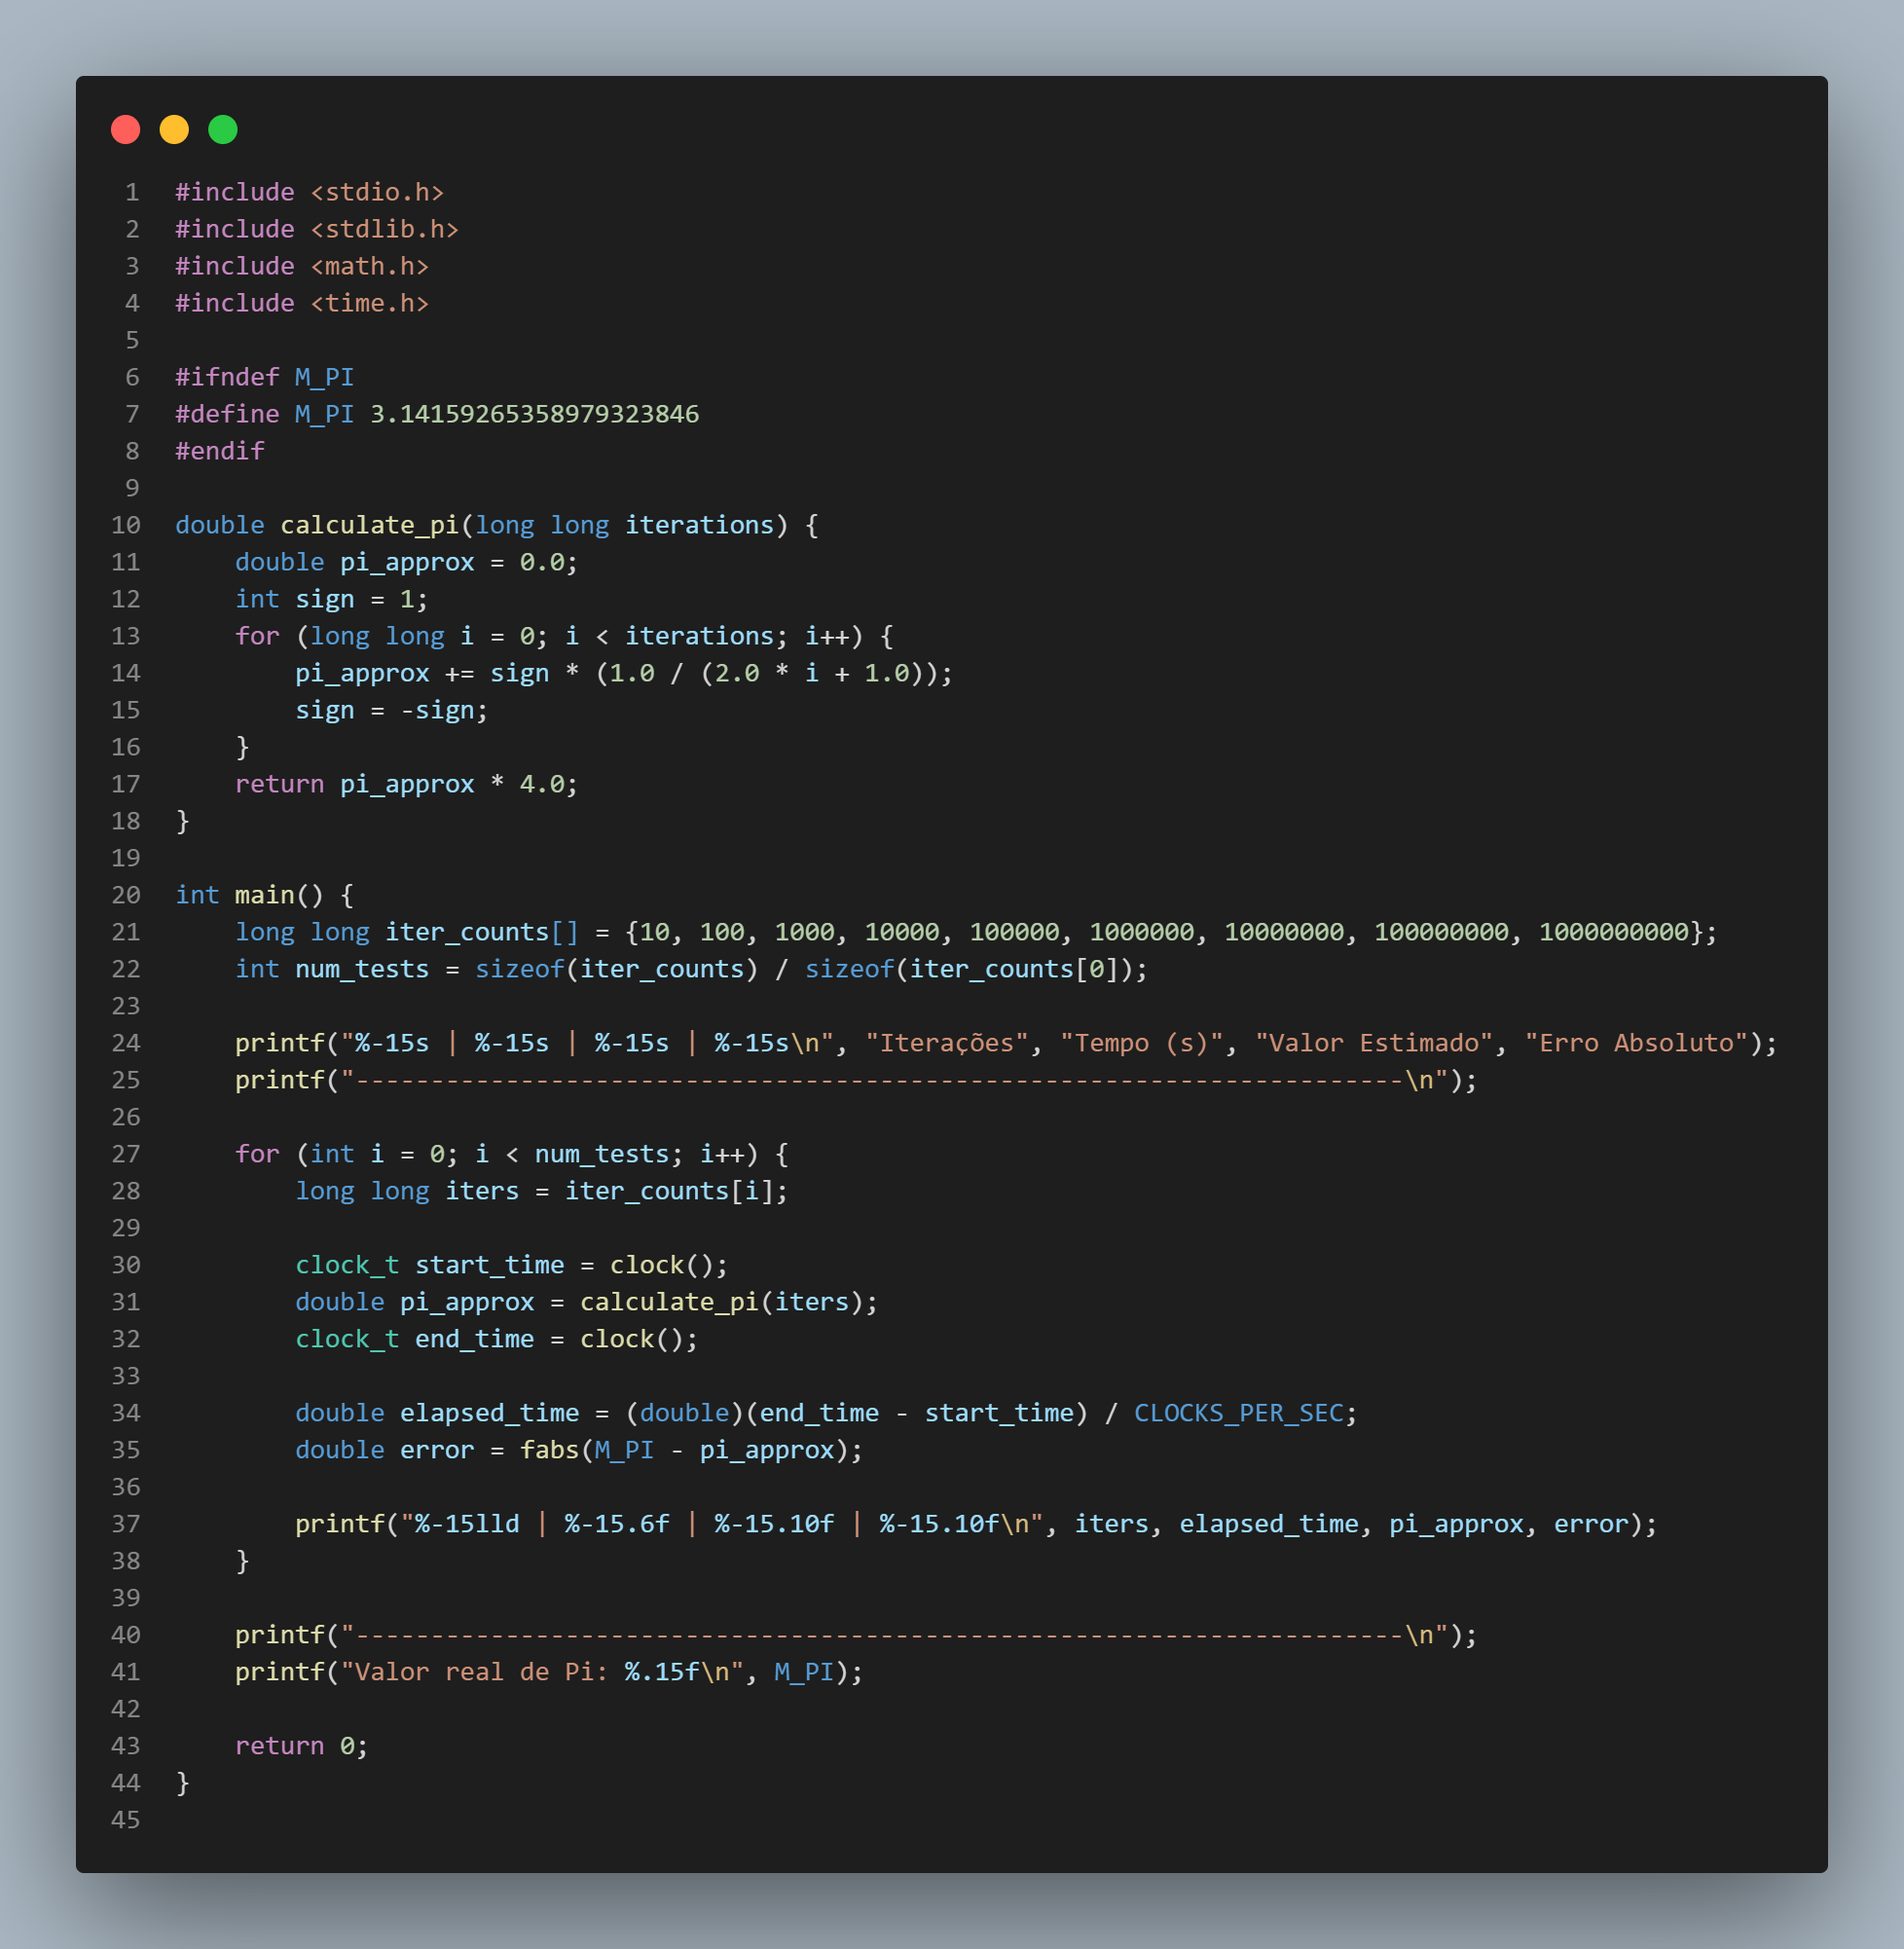
\includegraphics[width=\textwidth]{pi.png}
    \caption{Código-fonte da implementação da Série de Leibniz}
\end{figure}

\begin{lstlisting}
#include <stdio.h>
#include <stdlib.h>
#include <math.h>
#include <time.h>

#ifndef M_PI
#define M_PI 3.14159265358979323846
#endif

double calculate_pi(long long iterations) {
    double pi_approx = 0.0;
    int sign = 1;
    for (long long i = 0; i < iterations; i++) {
        pi_approx += sign * (1.0 / (2.0 * i + 1.0));
        sign = -sign;
    }
    return pi_approx * 4.0;
}

int main() {
    long long iter_counts[] = {10, 100, 1000, 10000, 100000, 1000000, 10000000, 100000000, 1000000000};
    int num_tests = sizeof(iter_counts) / sizeof(iter_counts[0]);

    printf("%-15s | %-15s | %-15s | %-15s\n", "Iteracoes", "Tempo (s)", "Valor Estimado", "Erro Absoluto");
    printf("----------------------------------------------------------------------\n");

    for (int i = 0; i < num_tests; i++) {
        long long iters = iter_counts[i];
        
        clock_t start_time = clock();
        double pi_approx = calculate_pi(iters);
        clock_t end_time = clock();
        
        double elapsed_time = (double)(end_time - start_time) / CLOCKS_PER_SEC;
        double error = fabs(M_PI - pi_approx);
        
        printf("%-15lld | %-15.6f | %-15.10f | %-15.10f\n", iters, elapsed_time, pi_approx, error);
    }

    printf("----------------------------------------------------------------------\n");
    printf("Valor real de Pi: %.15f\n", M_PI);

    return 0;
}
\end{lstlisting}

\subsection{Algoritmo \texttt{pi\_machin.c} (Fórmula de Machin)}

\begin{figure}[H]
    \centering
    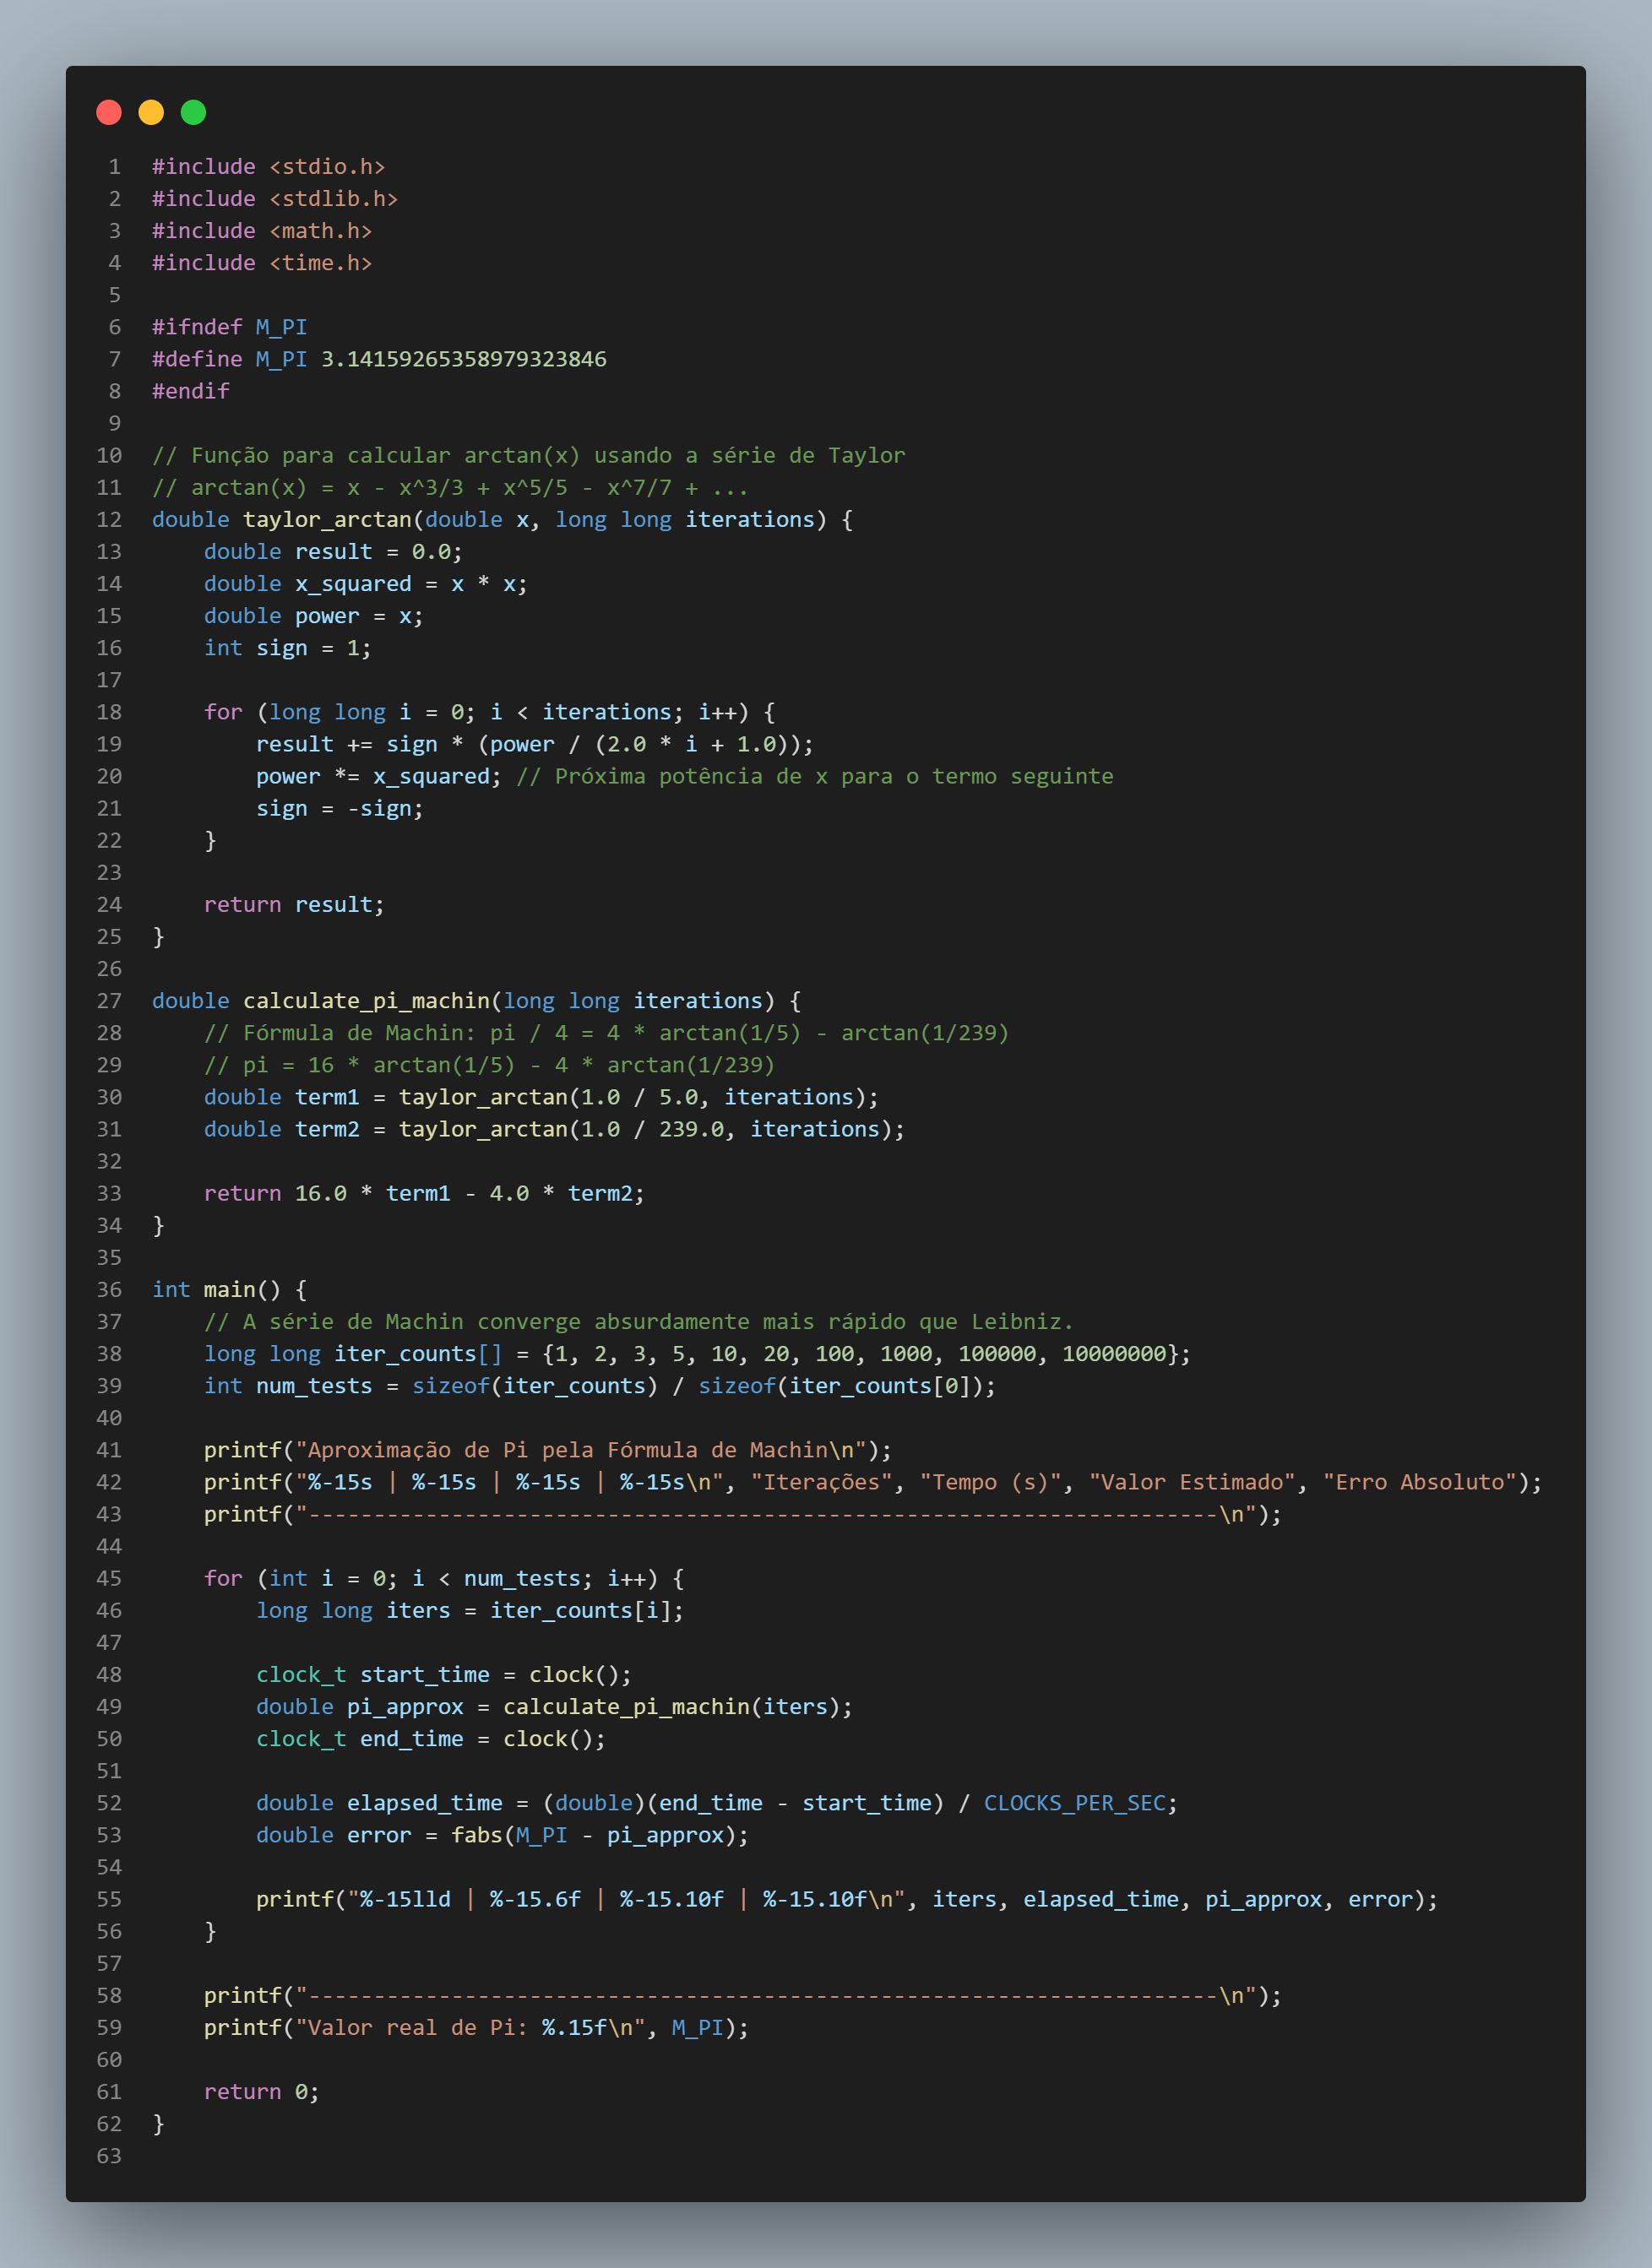
\includegraphics[width=\textwidth]{pi_machin.png}
    \caption{Código-fonte da implementação da Fórmula de Machin}
\end{figure}

\begin{lstlisting}
#include <stdio.h>
#include <stdlib.h>
#include <math.h>
#include <time.h>

#ifndef M_PI
#define M_PI 3.14159265358979323846
#endif

// Funcao para calcular arctan(x) usando a serie de Taylor
// arctan(x) = x - x^3/3 + x^5/5 - x^7/7 + ...
double taylor_arctan(double x, long long iterations) {
    double result = 0.0;
    double x_squared = x * x;
    double power = x;
    int sign = 1;

    for (long long i = 0; i < iterations; i++) {
        result += sign * (power / (2.0 * i + 1.0));
        power *= x_squared; // Proxima potencia de x para o termo seguinte
        sign = -sign;
    }
    
    return result;
}

double calculate_pi_machin(long long iterations) {
    // Formula de Machin: pi / 4 = 4 * arctan(1/5) - arctan(1/239)
    // pi = 16 * arctan(1/5) - 4 * arctan(1/239)
    double term1 = taylor_arctan(1.0 / 5.0, iterations);
    double term2 = taylor_arctan(1.0 / 239.0, iterations);
    
    return 16.0 * term1 - 4.0 * term2;
}

int main() {
    // A serie de Machin converge absurdamente mais rapido que Leibniz.
    long long iter_counts[] = {1, 2, 3, 5, 10, 20, 100, 1000, 100000, 10000000};
    int num_tests = sizeof(iter_counts) / sizeof(iter_counts[0]);

    printf("Aproximacao de Pi pela Formula de Machin\n");
    printf("%-15s | %-15s | %-15s | %-15s\n", "Iteracoes", "Tempo (s)", "Valor Estimado", "Erro Absoluto");
    printf("----------------------------------------------------------------------\n");

    for (int i = 0; i < num_tests; i++) {
        long long iters = iter_counts[i];
        
        clock_t start_time = clock();
        double pi_approx = calculate_pi_machin(iters);
        clock_t end_time = clock();
        
        double elapsed_time = (double)(end_time - start_time) / CLOCKS_PER_SEC;
        double error = fabs(M_PI - pi_approx);
        
        printf("%-15lld | %-15.6f | %-15.10f | %-15.10f\n", iters, elapsed_time, pi_approx, error);
    }

    printf("----------------------------------------------------------------------\n");
    printf("Valor real de Pi: %.15f\n", M_PI);

    return 0;
}
\end{lstlisting}

\end{document}
